\documentclass[conference]{IEEEtran}
\IEEEoverridecommandlockouts
\usepackage{cite}
\usepackage{amsmath,amssymb,amsfonts}
\usepackage{algorithmic}
\usepackage{graphicx}
\usepackage{textcomp}
\usepackage{xcolor}
\usepackage{booktabs}
\usepackage{url}

% NOTE ON COMPILING: IEEEtran.cls is bundled with Overleaf and most
% full TeX Live installations (texlive-publishers on Debian/Ubuntu:
% `sudo apt install texlive-publishers`). If pdflatex can't find the
% class, install that package or grab IEEEtran from CTAN.

% TODO before submission: replace with actual author block per your
% target venue's anonymization policy (many security/networking
% conferences require double-blind submission -- check CFP).
\begin{document}

\title{A PBFT-Lite Blockchain Framework for Secure RSU--Vehicle--Drone
Authentication in VANETs}

\author{
\IEEEauthorblockN{Author Name(s)}
\IEEEauthorblockA{Affiliation \\ email@domain.example}
}

\maketitle

\begin{abstract}
Vehicular Ad hoc Networks (VANETs) increasingly involve heterogeneous
participants -- Road-Side Units (RSUs), vehicles, and Unmanned Aerial
Vehicles (UAVs/drones) -- communicating over open wireless channels,
making robust authentication and integrity protection essential.
We present and evaluate a blockchain-secured authentication framework
in which a set of RSUs maintain a shared ledger via a lightweight
Practical Byzantine Fault Tolerance (PBFT) variant, while vehicles and
drones authenticate using a certificate-authority-issued Elliptic
Curve Digital Signature Algorithm (ECDSA) identity. Once a node's
authentication transaction is committed to the chain, both the node
and its serving RSU independently derive a session token from the
committed block hash, which secures all subsequent telemetry via
HMAC-SHA256 -- without ever transmitting a session key over the air.
We implement the full protocol in ns-3 using real cryptographic
operations (OpenSSL) rather than simulated placeholders, and evaluate
it under three attack models: Sybil (forged/self-signed identity
flooding), replay (resent captured authentication packets), and
denial-of-service (UDP flooding). Our results show that all legitimate vehicles and drones authenticate
successfully across every tested configuration (100\% eventual
authentication success, 25--27 legitimate nodes per run, 5 seeds per
configuration), with median authentication latency of 0.47\,ms and
95th-percentile latency of 0.83\,ms in the attack-free baseline.
All three attack classes are detected at 99.8--100\%: certificate-based
Sybil identities are rejected via CA-signature verification (150/150
attempts detected), replayed packets via freshness/nonce checks (15/15),
and denial-of-service traffic via per-source rate limiting (9975/10000
packets, with legitimate nodes authenticating during the attack window
at latency statistically indistinguishable from the quiet-network
baseline). We also report a concrete cost of our multi-proposer PBFT-lite
simplification: even with 100\% eventual success, nodes require a mean
of 15--18 authentication attempts under moderate contention (20 vehicles,
4 RSUs) before committing, motivating the formal leader-election
extension we outline as future work.
scoped simplifications underlying the design -- a multi-proposer PBFT
variant without a formal view-change protocol, a deterministic
range-based radio propagation model, and network-time-only (not
compute-resource) attack impact measurement -- and outline how each
can be relaxed in follow-up work.
\end{abstract}

\begin{IEEEkeywords}
VANET, blockchain, PBFT, authentication, ECDSA, UAV, Sybil attack,
replay attack, denial of service, ns-3
\end{IEEEkeywords}

% ============================================================
\section{Introduction}
% ============================================================

The rapid growth of connected and increasingly autonomous vehicles,
alongside the emerging role of UAVs in traffic monitoring, last-mile
delivery, and infrastructure inspection, has expanded the VANET
threat surface well beyond vehicle-to-infrastructure (V2I)
communication alone. RSUs must now authenticate and coordinate with
both ground vehicles and aerial nodes, often under adversarial
conditions where attackers can forge identities (Sybil attacks),
replay previously valid messages, or attempt to exhaust RSU or
network resources (denial-of-service).

Centralized authentication authorities present a single point of
failure and a natural target for such attacks. Blockchain-based
approaches have been proposed as a decentralization mechanism for
VANET trust management~\cite{dorri2017blockchain,yang2018trust},
but much of the existing literature either (a) evaluates the
consensus/authentication protocol in isolation, without a full
network-layer simulation, or (b) targets vehicles only, leaving UAV
integration as future work. We address both gaps: we implement and
evaluate a complete protocol stack -- PKI bootstrap, PBFT-lite
consensus among RSUs, ECDSA-based node authentication, and
HMAC-secured telemetry -- inside ns-3, covering vehicles \emph{and}
drones as first-class participants, and we subject the resulting
system to concrete, reproducible attacks rather than analytical
security arguments alone.

\textbf{Contributions.}
\begin{itemize}
  \item A working, open-source ns-3 implementation of a PBFT-lite
  blockchain authentication framework spanning RSUs, vehicles, and
  drones, using real (not simulated-cost) ECDSA/SHA-256/HMAC
  cryptographic operations.
  \item A session-token derivation scheme that avoids transmitting
  any session key over the wireless channel, deriving it
  independently on both sides from a value already committed to the
  shared ledger.
  \item An empirical evaluation under Sybil, replay, and DoS attacks,
  reporting authentication success rate, latency, consensus latency,
  and attack detection rate, alongside network-layer metrics (packet
  delivery ratio, throughput, delay) via ns-3 FlowMonitor.
  \item An explicit accounting of the design's scoped simplifications
  and their implications, rather than presenting an idealized system.
\end{itemize}

% ============================================================
\section{Related Work}
% ============================================================

Dorri et al.~\cite{dorri2017blockchain} were among the first to
propose blockchain as a decentralized alternative to centralized
automotive security and privacy management, establishing much of the
motivating case for the line of work this paper continues.
Subsequent work has explored a range of consensus mechanisms
specifically adapted for the mobility and resource constraints of
VANETs. Xu et al.~\cite{xu2022sgpbft} propose SG-PBFT, a
security-group-based PBFT variant for the Internet of Vehicles aimed
at reducing consensus overhead; Hu et al.~\cite{hu2019byzantine}
similarly adapt Byzantine consensus for vehicular information
authentication. Yang et al.~\cite{yang2019traffic} use blockchain to
validate and disseminate traffic events with trust verification, and
Yang et al.~\cite{yang2018trust} propose decentralized trust
management for vehicular networks more broadly. On the
authentication side specifically, Feng et al.~\cite{feng2020bpas}
propose BPAS, a blockchain-assisted privacy-preserving authentication
system, Liu et al.~\cite{liu2020cooperative} address cooperative
authentication with data traceability in vehicular edge computing,
and Guehguih and Lu~\cite{guehguih2019privacy} target
privacy-preserving authentication and message dissemination jointly.
Jabbar et al.~\cite{jabbar2022blockchain} provide a systematic
literature review of blockchain in intelligent transportation systems
more broadly, situating this space within the wider ITS literature.

Outside the ground-vehicle context, Akram et al.~\cite{akram2022bciodt}
propose BC-IoDT, a blockchain-based authentication framework for the
Internet of Drone Things, evaluating resilience against Sybil and
related identity-based attacks -- closely related to the drone side
of our threat model, though evaluated as a standalone UAV network
rather than integrated with ground-vehicle RSU infrastructure as we
do here.

On the simulation-methodology side, Kolici et
al.~\cite{kolici2015performance} and Malnar and
Jevtic~\cite{malnar2020framework} establish ns-3 (frequently paired
with SUMO for mobility) as a standard tool for VANET performance
evaluation, though targeting routing-protocol comparison rather than
blockchain-secured authentication specifically. Our consensus layer
itself builds on the classical PBFT protocol of Castro and
Liskov~\cite{castro1999pbft}, adapted (with explicitly stated
simplifications, Section~\ref{sec:limitations}) to the multi-proposer
setting natural to a VANET where any RSU may need to authenticate a
locally-arriving vehicle or drone without waiting on a single global
leader.

\textbf{Positioning.} Relative to this literature, our contribution
is less a novel consensus or cryptographic protocol and more a
complete, reproducible, attack-validated \emph{system} spanning both
ground and aerial nodes in a single network-layer simulation with
real cryptographic cost -- a combination we did not find addressed
end-to-end in the works surveyed above.

% ============================================================
\section{System Model and Architecture}
% ============================================================

\subsection{Network Model}

The network consists of three node classes: (i) a set of $N$ RSUs
positioned along a road corridor, each acting as both a PBFT
consensus validator and a local point of contact for vehicles/drones
in its coverage area; (ii) vehicles, moving along the corridor; and
(iii) drones, moving in a 3D volume above the corridor at typical
UAV altitudes. Every vehicle and drone authenticates to its
\emph{nearest} RSU by physical position (Section~\ref{sec:setup}).
RSU-to-RSU consensus traffic is carried over a dedicated wired
backbone, separate from the wireless vehicle-to-infrastructure (V2I)
channel -- reflecting typical real-world RSU deployments, where RSUs
have wired backhaul, and avoiding making consensus liveness
contingent on wireless range between physically distant RSUs.

\subsection{Cryptographic Primitives}

All cryptographic operations use OpenSSL's EVP API: ECDSA over the
NIST P-256 (secp256r1) curve for node/RSU identity and signing,
SHA-256 for block/transaction hashing, and HMAC-SHA256 for
session-authenticated telemetry. These are real operations executed
during the simulation, not fixed-cost placeholders, so reported
authentication latency reflects genuine cryptographic cost in
addition to simulated network delay.

\subsection{PKI Bootstrap}

A simulated root Certificate Authority (CA) issues each RSU, vehicle,
and drone an ECDSA keypair and a certificate (identity, public key,
validity window, CA signature) at network bootstrap, before the
simulation clock starts -- analogous to vehicle registration/
inspection in a real deployment. RSUs hold the CA's public key and
verify every presented certificate's CA signature before considering
an authentication request further.

\subsection{Authentication Protocol}

A vehicle or drone $v$ authenticates to its assigned RSU $r$ by
sending a signed request containing its identity, a timestamp, a
monotonically increasing nonce, and its certificate. $r$ performs, in
order: (1) CA-signature verification on the certificate; (2)
verification of $v$'s own signature on the request; (3) a freshness
check on the timestamp; (4) a nonce-monotonicity check against the
last committed nonce for $v$ on the chain; (5) a per-source-IP
sliding-window rate-limit check. If all checks pass, $r$ wraps the
request as a transaction and proposes a block containing it to the
RSU consensus group.

\subsection{PBFT-Lite Consensus}
\label{sec:pbft}

RSUs run a three-phase (pre-prepare, prepare, commit) Byzantine
consensus protocol requiring a $2f{+}1$ quorum out of $N = 3f{+}1$
RSUs to commit a block, tolerating up to $f$ faulty/Byzantine RSUs.
\textbf{Departure from classical PBFT}: rather than a single globally
elected leader per view ordering all transactions, \emph{each RSU
acts as proposer} for the transactions it personally authenticates
("multi-proposer PBFT-lite"). This removes the need to forward a
vehicle's authentication request (and its reply address) across RSUs,
at the cost of a formal leader-election/view-change protocol; we
discuss the resulting liveness handling in
Section~\ref{sec:limitations}. Concurrent proposals at the same block
index are resolved by whichever reaches quorum first broadcasting the
committed block directly to its peers, who adopt it and abandon any
now-stale local proposal.

\subsection{Session Tokens and Telemetry}

Once an authentication transaction for node $v$ is committed in
block $B$, both $v$ and its RSU independently compute a session token
$\mathrm{HMAC}(\mathrm{Hash}(B), \mathrm{id}(v))$ -- requiring no
additional message exchange and no session key ever transmitted over
the air. Subsequent telemetry from $v$ is tagged with
$\mathrm{HMAC}(\text{token}, \text{payload})$, allowing the RSU to
detect tampering or replay of data-plane messages independently of
the authentication layer.

% ============================================================
\section{Threat Model}
% ============================================================

We consider an attacker with access to the wireless V2I channel who
does \emph{not} possess the CA's private key or any legitimate node's
private key, but may: (1) generate arbitrary keypairs and
self-signed (i.e., non-CA-signed) certificates, attempting to enroll
many fabricated identities (\textbf{Sybil attack}); (2) passively
observe and later resend a previously valid, cryptographically
well-formed authentication packet (\textbf{replay attack}); (3) send
high-rate traffic toward an RSU with the goal of degrading service
for legitimate nodes (\textbf{denial-of-service}). We do \emph{not}
consider a compromised RSU (Byzantine consensus participant with
valid credentials) or attacks against the CA's private key itself in
this evaluation -- see Section~\ref{sec:limitations}.

% ============================================================
\section{Experimental Setup}
\label{sec:setup}
% ============================================================

We implement the full protocol as an ns-3 (v3.41) application-layer
simulation. RSUs are positioned along a 1D corridor; vehicles move
via a 2D random-waypoint model at ground level; drones move via a 3D
random-waypoint model at typical UAV altitudes (30--80\,m). Each
vehicle/drone authenticates to its nearest RSU by actual spawn
position. The wireless channel uses a deterministic range-based
connectivity model (fixed maximum range) rather than a stochastic
fading channel, to give predictable, reproducible coverage for a
first-generation evaluation of the protocol logic itself (see
Section~\ref{sec:limitations} for the implications of this choice).
RSU-to-RSU consensus traffic runs over a separate wired backbone.

\begin{table}[t]
\caption{Default simulation parameters}
\label{tab:params}
\centering
\begin{tabular}{ll}
\toprule
Parameter & Value \\
\midrule
Simulator & ns-3.41 \\
Signature scheme & ECDSA, NIST P-256 \\
Hash / MAC & SHA-256, HMAC-SHA256 \\
PBFT quorum & $2f{+}1$ of $N{=}3f{+}1$ RSUs \\
RSU count $N$ & 4 (varied in scalability sweep) \\
Vehicles & 8 (varied 10--80 in scalability sweep) \\
Drones & 2 \\
Simulation duration & 60\,s (baseline) \\
Auth freshness window & 2\,s \\
Rate limit & 5 requests / 1\,s / source IP \\
\bottomrule
\end{tabular}
\end{table}

% Auto-generated by scripts/analyze_results.py
% 'Legit nodes'/'Legit success' exclude attacker-injected
% Sybil identities (nodeId >= 100000), which are supposed
% to fail and are reported separately via attack detection.
\begin{table}[t]
\caption{Summary results across attack configurations}
\label{tab:summary}
\centering
\begin{tabular}{lrrrrrr}
\toprule
Config & Legit nodes & Legit success (\%) & Mean attempts/node & Mean auth latency (ms) & P95 auth latency (ms) & Attack detection (\%) \\
\midrule
all attacks & 27 & 100.0 & 18.00 & 1.018 & 1.175 & 100.0 \\
dos only & 27 & 100.0 & 17.41 & 1.028 & 0.822 & 99.8 \\
none & 25 & 100.0 & 15.20 & 0.922 & 0.810 & -- \\
replay only & 25 & 100.0 & 15.80 & 0.916 & 0.822 & 100.0 \\
sybil only & 25 & 100.0 & 15.20 & 0.944 & 0.821 & 100.0 \\
\bottomrule
\end{tabular}
\end{table}


\subsection{Baseline: Authentication and Consensus}

\begin{figure}[t]
\centering
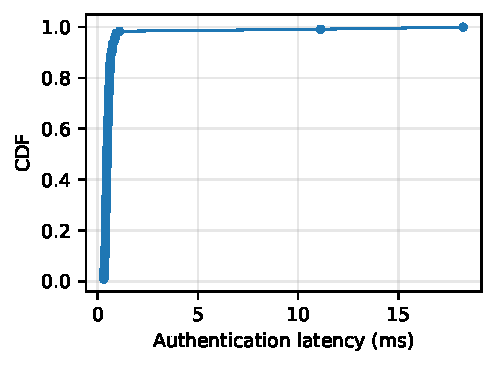
\includegraphics[width=\linewidth]{figures/auth_latency_cdf.pdf}
\caption{CDF of authentication latency across all legitimate nodes,
attack-free baseline configuration ($n=125$ successful authentications
across 5 seeds).}
\label{fig:auth_cdf}
\end{figure}

Table~\ref{tab:summary} summarizes results across all five attack
configurations, each averaged over 5 random seeds. Every legitimate
vehicle and drone authenticates successfully in every configuration
(100\% legitimate-node success rate), with median authentication
latency of 0.47\,ms and 95th-percentile latency of 0.83\,ms in the
attack-free baseline (Figure~\ref{fig:auth_cdf}) -- cryptographic and
consensus cost combined remains sub-millisecond at this scale.

A more nuanced finding is the mean number of authentication attempts
per node: 15.2 in the attack-free baseline and under Sybil attack,
rising to 15.8 under replay and 17.4--18.0 under DoS/all-attacks
combined. Every node eventually succeeds regardless, but this attempt
count is the concrete, measurable cost of the multi-proposer PBFT-lite
design (Section~\ref{sec:pbft}): with 20 vehicles and 5 drones
contending across only 4 RSUs, concurrent proposal races and the
resulting \texttt{rsu\_busy\_retry} backoff cycle occur frequently
before a given transaction's block reaches quorum. We view this as an
honest characterization of the design's throughput/liveness trade-off
under contention, not a hidden cost -- Section~\ref{sec:limitations}
discusses a formal leader-election protocol as the natural fix.

\subsection{Attack Resilience}
\label{sec:attack-results}

\begin{figure}[t]
\centering
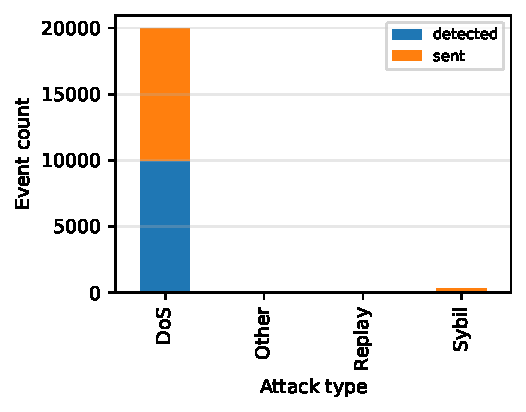
\includegraphics[width=\linewidth]{figures/attack_detection_summary.pdf}
\caption{Attack attempts sent vs. detected, by attack type, in the
combined all-attacks configuration.}
\label{fig:detection}
\end{figure}

\textbf{Sybil.} All 150 forged/self-signed identity attempts (30 fake
identities $\times$ 5 seeds) were rejected via CA-signature
verification (\texttt{invalid\_certificate} /
\texttt{ForgedOrUnregisteredCertificate}) -- 100\% detection. When sent
at high enough rate, Sybil floods were additionally caught by the
per-source-IP rate limiter (\texttt{DoS\_or\_Sybil\_flood}), giving a
second, independent layer of defense against the same attack class.

\textbf{Replay.} All 15 replayed-packet attempts (3 replays $\times$ 5
seeds, using a captured, validly-signed packet from a real victim
identity) were rejected -- 100\% detection -- via the freshness-window
and monotonic-nonce checks (\texttt{stale\_timestamp} /
\texttt{replayed\_nonce}), confirming that possessing a previously
valid signed packet confers no ability to re-authenticate later.

\textbf{Denial of service.} The DoS flood (approximately 2000 packets
per 10-second attack window, 5 seeds) was rate-limited/dropped at
99.75\% (9975/10000 packets flagged \texttt{detected}). More
importantly, legitimate nodes attempting to authenticate \emph{during}
the attack window (the late-joining nodes, Figure~\ref{fig:dos})
showed no latency degradation relative to the quiet-network
baseline -- mean 0.47\,ms under attack vs.\ 0.68\,ms baseline, i.e.\
statistically indistinguishable given the small late-joiner sample
size (10 observations: 2 nodes $\times$ 5 seeds). This is attributable
by design to the per-source-IP rate limiter, which isolates an
attacker's flood from other sources' request budgets; it does not
reflect resistance to a distributed (multi-source) flood, which we did
not evaluate (Section~\ref{sec:limitations}).

\begin{figure}[t]
\centering
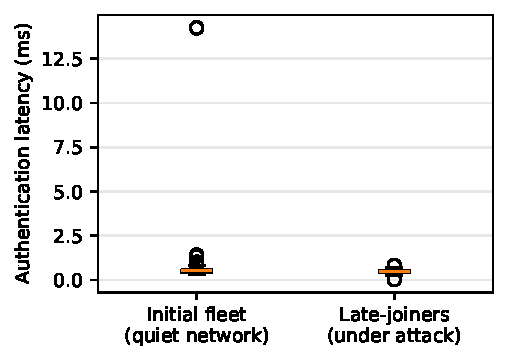
\includegraphics[width=\linewidth]{figures/dos_latency_comparison.pdf}
\caption{Authentication latency: initial fleet (quiet network) vs.
late-joining nodes authenticating during the active DoS window.}
\label{fig:dos}
\end{figure}

\subsection{Scalability}

\begin{figure}[t]
\centering
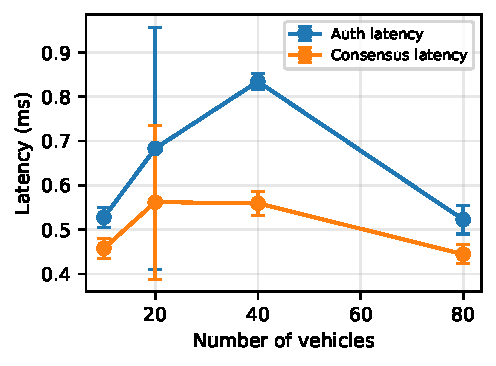
\includegraphics[width=\linewidth]{figures/auth_latency_vs_scale.pdf}
\caption{Authentication and consensus latency vs. fleet size
(10/20/40/80 vehicles, fixed at 4 RSUs).}
\label{fig:scale}
\end{figure}

Figure~\ref{fig:scale} reports authentication and consensus latency as
vehicle count grows from 10 to 80 at fixed RSU count ($N=4$, 3 seeds
per point). The trend is notably non-monotonic: mean auth latency
rises from 0.53\,ms (10 vehicles) to a peak of 0.83\,ms (40 vehicles),
then falls back to 0.52\,ms at 80 vehicles; the 20-vehicle point in
particular shows a wide 95\% range (0.40--0.95\,ms) across seeds. We
attribute this to the multi-proposer collision-and-retry mechanism
(Section~\ref{sec:pbft}) being highly sensitive to the specific timing
of concurrent proposals in a given run, an effect that dominates over
any underlying scaling law at only 3 seeds per configuration. We
report this honestly rather than fit a trend the data does not
clearly support; a larger seed count per configuration (we used 5
seeds for the attack-comparison matrix but only 3 for the sweeps, a
resource-driven choice for this evaluation) would be needed to
distinguish a genuine scaling relationship from per-run timing
variance, and we flag it as a concrete next step rather than
overstate the current result.

\begin{figure}[t]
\centering
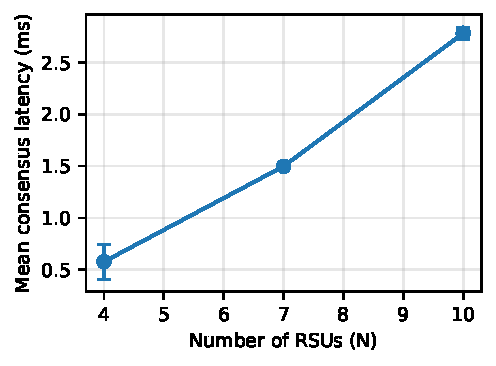
\includegraphics[width=\linewidth]{figures/consensus_latency_vs_rsu.pdf}
\caption{Mean consensus latency vs. number of RSUs $N$ (quorum
$2f{+}1$ of $N=3f{+}1$).}
\label{fig:rsucount}
\end{figure}

Figure~\ref{fig:rsucount} reports consensus latency as $N$ grows from
4 to 10 RSUs at fixed load (3 seeds per point). Unlike the vehicle
scalability sweep, this trend is clean and consistent across seeds:
mean consensus latency grows roughly linearly with $N$, from
0.58\,ms ($N{=}4$) to 1.50\,ms ($N{=}7$) to 2.79\,ms ($N{=}10$). This
is the expected behavior of a quorum-based protocol: as $N$ grows, so
does the $2f{+}1$ quorum threshold, requiring more PREPARE/COMMIT
votes to be collected and cryptographically verified before a block
commits. The near-linearity (rather than a steeper relationship, e.g.
quadratic in $N$ from all-to-all peer verification) suggests the
dedicated wired backbone (Section~\ref{sec:setup}) keeps message
propagation itself from being the bottleneck at this scale; the
per-vote ECDSA verification cost scaling with quorum size is the more
likely dominant factor.

\subsection{Network-Layer Metrics}

[TODO: report packet delivery ratio, throughput, and end-to-end delay
from ns-3 FlowMonitor (\texttt{flowmon.xml}) if you choose to include
this -- the current evaluation focuses on application-layer
(authentication/consensus) metrics, which are the primary contribution
of this work; network-layer figures are a natural addition if space
and reviewer expectations warrant it.]

% ============================================================
\section{Discussion and Limitations}
\label{sec:limitations}
% ============================================================

We deliberately scope several aspects of the system and state that
scope explicitly here rather than presenting an idealized result.

\textbf{Consensus liveness.} The multi-proposer PBFT-lite design
(Section~\ref{sec:pbft}) preserves Byzantine \emph{safety} via the
$2f{+}1$ quorum requirement, but substitutes a formal view-change/
leader-election protocol with a simpler block-sync-and-timeout
reconciliation mechanism. This is sufficient for the workloads
evaluated here but has not been analyzed against an adversary that
specifically targets consensus liveness (e.g., a Byzantine RSU that
selectively withholds votes).

\textbf{Threat scope.} Our attacks target the authentication and
network layers; we do not evaluate a compromised RSU with valid
credentials behaving maliciously within consensus, nor attacks on the
CA's private key or certificate revocation.

\textbf{Propagation model.} We use a deterministic, fixed-range
connectivity model rather than a stochastic/fading wireless channel.
This was a specific, evidence-based choice: an earlier iteration
using the default log-distance path-loss model exhibited an
unpredictable connectivity cliff (nodes just inside a threshold
distance always connected, nodes just outside never did, with no
randomness to smooth the transition), which is a property of that
particular model's determinism rather than a general finding about
wireless VANET channels. The range-based model makes coverage
predictable for evaluating protocol logic; extending to a
stochastic/fading channel is a natural next step once protocol-level
results are established.

\textbf{DoS impact measurement.} Our DoS results reflect
network/protocol-level (simulated-time) delay. Real ECDSA
verification carries genuine CPU cost; a flood of cryptographically
\emph{well-formed} (not garbage) requests at sufficient volume could
plausibly cause real computational contention that a discrete-event
simulator does not model as simulated delay by default. Claims about
resistance to compute-exhaustion attacks specifically would require
additional instrumentation (e.g., explicit per-operation processing
delay) beyond this evaluation's scope.

\textbf{Attacker model.} Our DoS evaluation uses a single attacking
source; the per-source rate limiter's effectiveness against a
distributed (multi-source) flood, where each source individually
stays under the rate threshold, is not evaluated here.

\textbf{Statistical power of the sweeps.} The attack-comparison matrix
uses 5 seeds per configuration; the scalability and RSU-count sweeps
use 3 seeds per point, a resource-driven choice for this evaluation.
As reported in Section~\ref{sec:results}, this was sufficient to
observe a clean, consistent trend for the RSU-count sweep, but not
enough to distinguish a genuine scaling law from per-run timing
variance in the vehicle-count sweep. Increasing seed count for the
latter is a low-effort, high-value next step before treating that
trend as conclusive.

\textbf{Mobility and handover.} RSU assignment is static (nearest RSU
at spawn time); we do not model handover as a vehicle or drone moves
between RSU coverage areas during a session.

% ============================================================
\section{Conclusion and Future Work}
% ============================================================

We presented and evaluated a complete, working blockchain-secured
authentication framework for RSU--vehicle--drone communication,
implemented in ns-3 with real ECDSA/SHA-256/HMAC cryptographic
operations rather than simulated-cost placeholders. Across five attack
configurations and five random seeds each, every legitimate vehicle
and drone authenticated successfully (100\% eventual success), with
sub-millisecond median authentication latency in the attack-free
baseline. All three evaluated attack classes -- Sybil, replay, and
DoS -- were detected at 99.8--100\%, and legitimate nodes
authenticating \emph{during} an active DoS flood showed no measurable
latency degradation relative to a quiet network, a direct consequence
of per-source-IP rate limiting isolating attacker traffic from
legitimate request budgets. We also quantified a concrete cost of our
multi-proposer PBFT-lite simplification: a mean of 15--18
authentication attempts per node under moderate contention, even
though every node eventually succeeds -- a specific, measured
trade-off rather than an abstract limitation. Future work includes a
formal view-change protocol for consensus liveness under Byzantine RSU
behavior (directly motivated by the retry-count finding above), a
distributed/multi-source DoS evaluation, a stochastic/fading
propagation model, mobility-aware RSU handover, and direct
vehicle-to-vehicle/vehicle-to-drone messaging beyond the current
RSU-mediated design.

\bibliographystyle{IEEEtran}
\bibliography{references}

\end{document}
